\section{Properties of networks}
\label{sec:ch4:prop-net}


\subsection{Descriptive Properties of Networks}

Remember that with a network, we can represent the collection of nodes and edges as an $n \times n$ adjacency matrix, where $n$ is the total number of nodes. The adjacency matrix looks like this:

\begin{align*}
    A &= \begin{bmatrix}
        a_{11} & ... & a_{1n} \\
        \vdots & \ddots & \vdots \\
        a_{n1} & ... & a_{nn}
    \end{bmatrix},
\end{align*}

Let's say you have a network representing the five boroughs of New York (Staten Island SI, Brooklyn BK, Queens Q, the Bronx BX, and Manhattan MH). The nodes in your network are the five boroughs. The edges $(i,j)$ of your network exist if one can travel from borough $i$ to borough $j$ along a bridge. Let's start by defining a network for ourselves with \texttt{networkx}'s \texttt{DiGraph()} function:


\begin{lstlisting}[style=python]
import networkx as nx
from graphbook_code import heatmap

# create an undirected network G
G = nx.Graph()
# add the nodes like before
G.add_node("SI", pos=(2,1))
G.add_node("MH", pos=(4,4))
G.add_node("BK", pos=(4,1.7))
G.add_node("Q", pos=(6,3))
G.add_node("BX", pos=(6,6))

# specify boroughs that are connected to one another
pos = nx.get_node_attributes(G, 'pos')
G.add_edge("SI", "BK")
G.add_edge("MH", "BK")
G.add_edge("MH", "Q")
G.add_edge("MH", "BX")
G.add_edge("Q", "BX")

A = nx.to_numpy_array(G)

# plotting
nx.draw_networkx(G, with_labels=True, node_color="black", pos=pos,
                font_color="white", edge_color="black")

# pass in the xticklabels and yticklabels corresponding to the
# appropriately ordered boroughs (in the order we constructed them)
heatmap(A.astype(int), xticklabels=["SI", "MH", "BK", "Q", "BX"],
            yticklabels=["SI", "MH", "BK", "Q", "BX"], 
       ).set(xlabel="Borough", ylabel="Borough")
\end{lstlisting}

Figure \ref{fig:ch4:nyc_ex} shows a plot of the bridges of New York, a layout plot representation of a network derived from the the boroughs of New York, and an adjacency matrix as a heatmap of this network.

In this section, we're going to discuss a number of descriptive measures and summary statistics about networks. For a detailed overview, there are a lot of great references out there; some of our favorites are \cite{Barabsi2013Mar}, \cite{Gross2005Sep}, and \cite{Newman2006Jun}, to name a few.

\begin{figure}
    \centering
    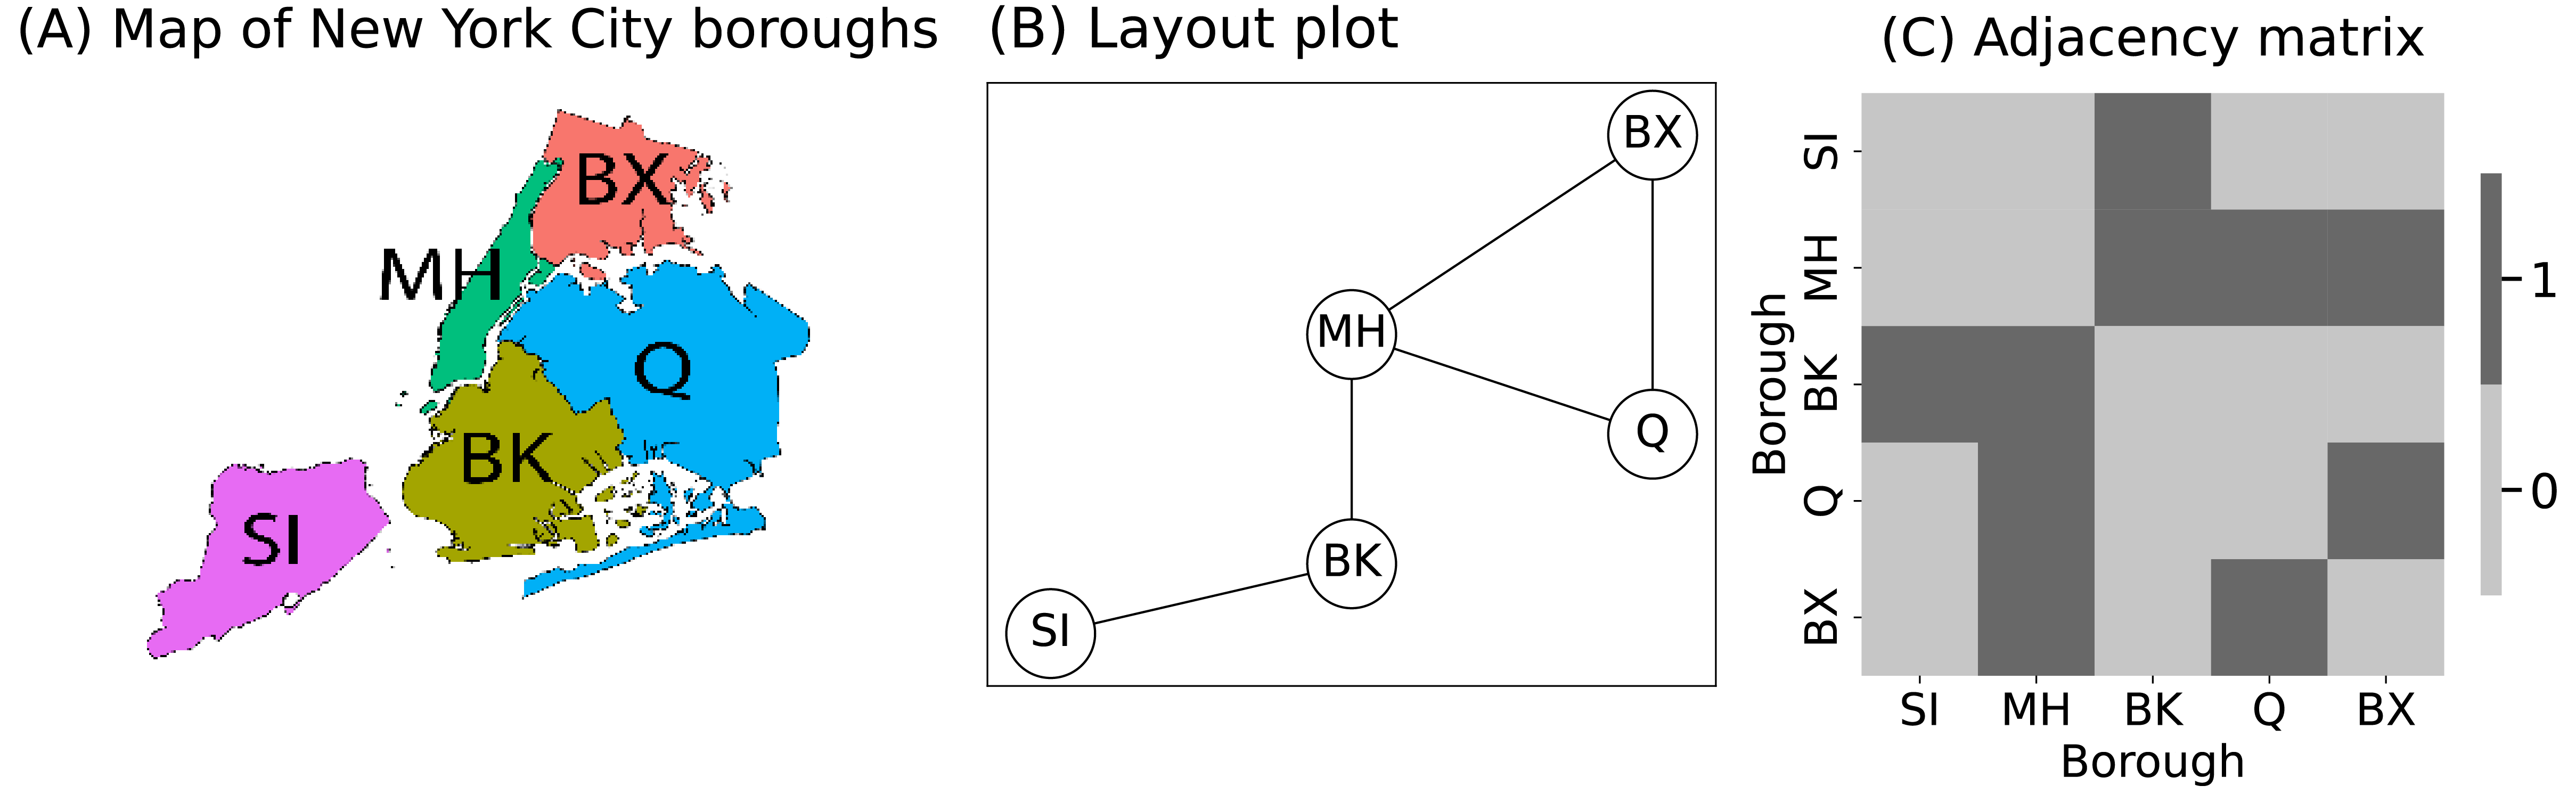
\includegraphics[width=\linewidth]{representations/ch4/Images/nyc_ex.png}
    \caption[New York City borough example]{\textbf{(A)} a map of New York, with the bridges that connect different boroughs. We use this to construct a network of New York, where the nodes are boroughs of New York and the edges are bridges between different boroughs. \textbf{(B)} the network visualized as a layout plot. \textbf{(C)} the network visualized as a heatmap.}
    \label{fig:ch4:nyc_ex}
\end{figure}

\subsection{The edges of undirected networks are bi-directional}

When you decide to travel from borough $i$ to borough $j$, you care about whether you can {actually drive} in that direction. In a similar way, the concept of directedness describes whether you need to worry about one-way bridges and bridge closures. If your network contains one-way bridges, then a bridge from borough $i$ to borough $j$ doesn't {necessarily} imply that a bridge from borough $j$ to borough $i$ exists (just ask New York drivers). If, for instance, the Brooklyn bridge was closed from Brooklyn to Manhattan, your network might change like this. Note that there is no arrow going from Brooklyn to Manhattan, so you cannot drive directly from MH to BK. We can do this by removing the edge from MH to BK:

\begin{lstlisting}[style=python]
from copy import deepcopy

G_dir = G.to_directed()
# remove the edge from MH to BK
G_dir.remove_edge("BK", "MH")

nx.draw_networkx(G_dir, with_labels=True, node_color="black", pos=pos,
                font_color="white", arrows=True, edge_color="black")
\end{lstlisting}

Basically, the arrows of the directed network tell you which nodes you can travel between. Note that we passed the \texttt{arrows="True"} argument, which tells \texttt{networkx} to include the arrows in our plot. A plot of this network is shown in Figure \ref{fig:ch4:directed}(B). Note that there are bi-directional arrows (arrows from one node to the other, as well as the reverse) for all pairs of nodes except Brooklyn and Manhattan.

\begin{figure}[h]
    \centering
    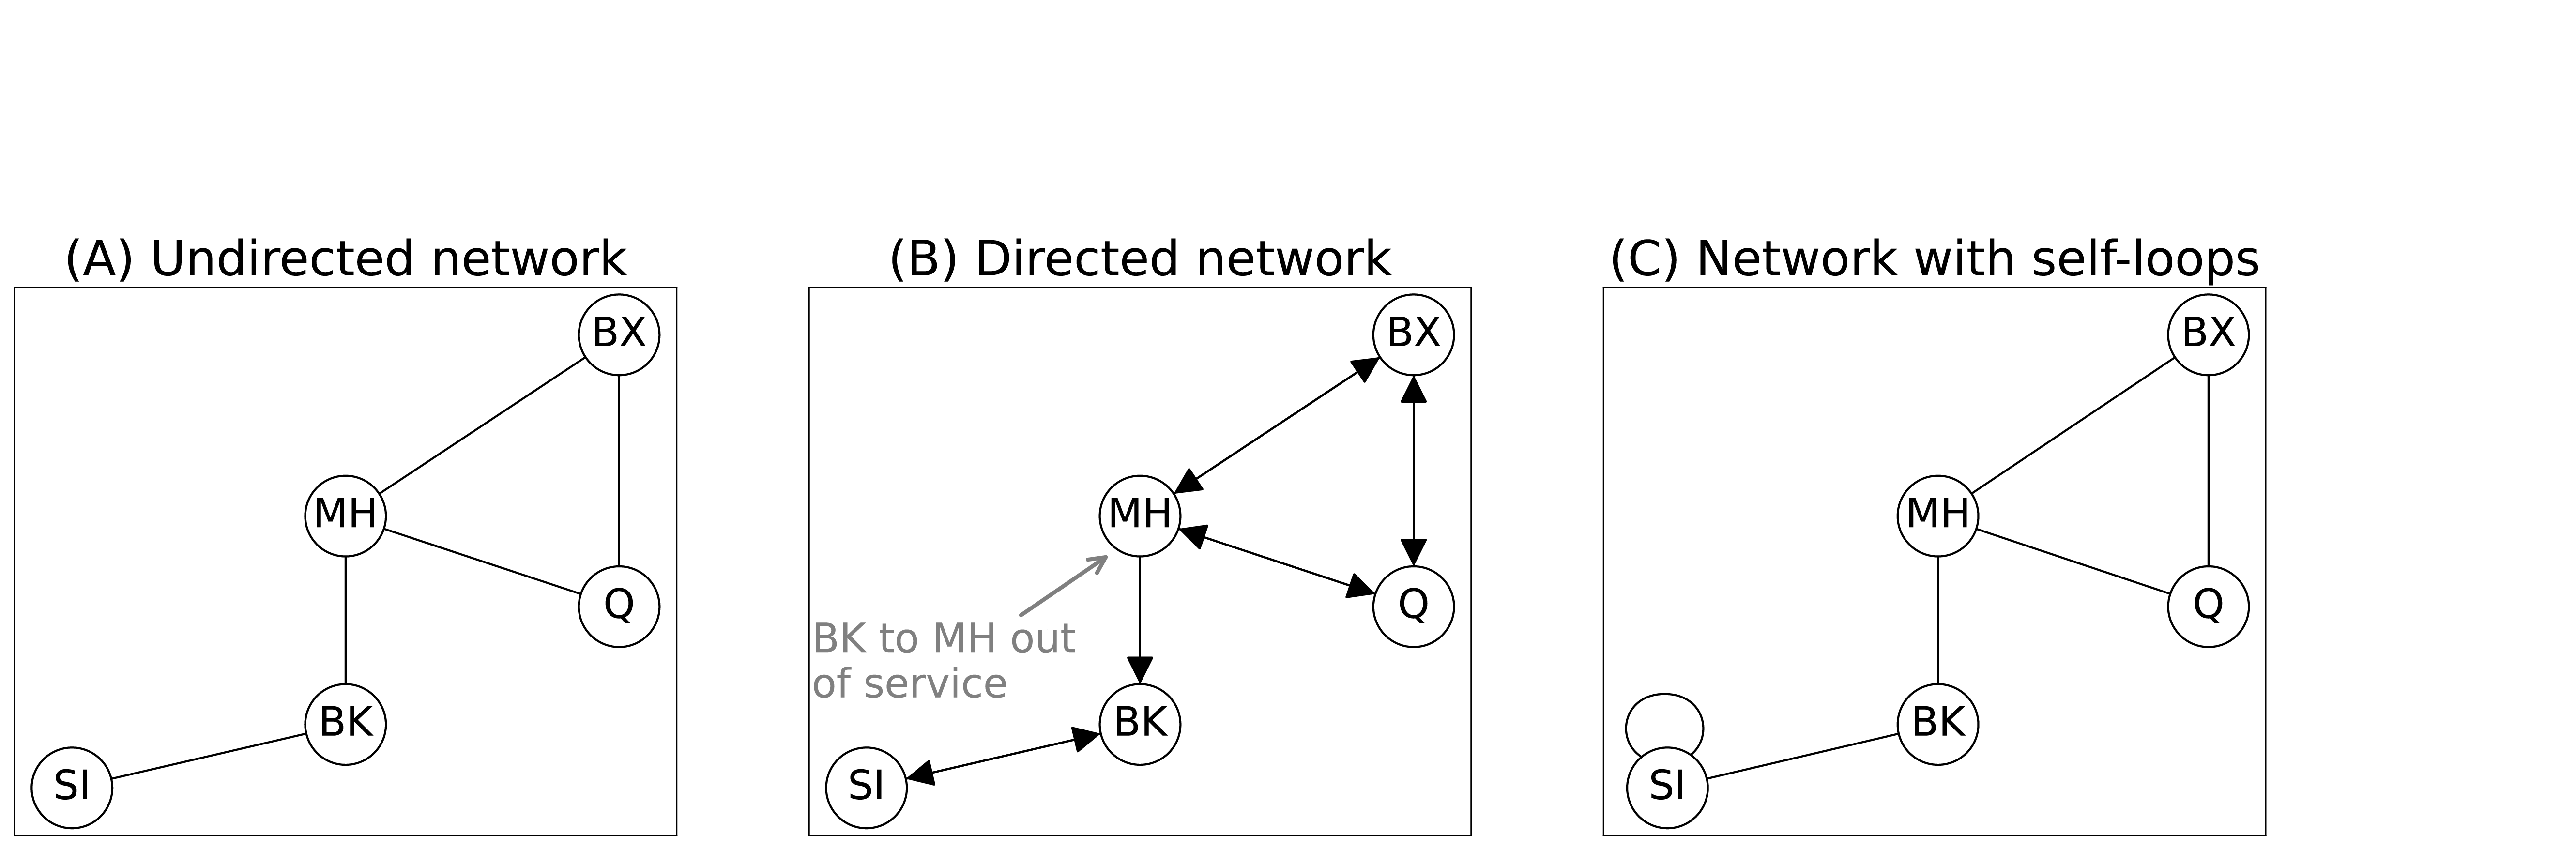
\includegraphics[width=\linewidth]{representations/ch4/Images/directed.png}
    \caption[Comparing directed and undirected networks]{\textbf{(A)} The undirected network. \textbf{(B)} A plot of the network with the bridge from BK to MH out of service. \textbf{(C)} a plot of the network with a self-loop.}
    \label{fig:ch4:directed}
\end{figure}

In the context of this book, we will usually only worry about the undirected case, or when the presence of an arrow implies that the other direction exists, too. A network is \textit{undirected} if an edge between node $i$ and node $j$ implies that node $j$ is also connected to node $i$. 

A plot of the undirected network is shown in Figure \ref{fig:ch4:directed}(A). For the adjacency matrix $A$, remember an edge between nodes $i$ and $j$ is represented by the adjacency $a_{ij}$. This means that if the network is undirected, $a_{ij} = a_{ji}$, for all pairs of nodes $i$ and $j$. By definition, this tells us that the adjacency matrix $A$ is \textit{symmetric}, so $A = A^\top$. We can verify this condition with \texttt{graspologic}:
\begin{lstlisting}[style=python]
from graspologic.utils import is_symmetric

A = nx.to_numpy_array(G)
is_symmetric(A)
# True
A_dir = nx.to_numpy_array(G_dir)
is_symmetric(A_dir)
# False
\end{lstlisting}

\subsubsection{Loopless networks do not have self-loops}

If you are already in a borough, why would you want to take a bridge to that same borough? This logic relates to the concept of {self-loops} in a network. A \textit{self-loop} in a network describes whether nodes can connect back to themselves. For instance, consider the following loop on Staten Island. This would have the interpretation of a bridge which connects Staten Island back to itself:
\begin{lstlisting}[style=python]
G_loopy = deepcopy(G)
# add edge from SI to itself
G_loopy.add_edge("SI", "SI")
nx.draw_networkx(G_loopy, with_labels=True, node_color="black", pos=pos,
                font_color="white", edge_color="black")
\end{lstlisting}

A plot of this network is shown in Figure \ref{fig:ch4:directed}(C). A network is \textit{loopless} if self-loops are not possible. It is also important to note that both directed and undirected network can have self-loops; we only show the undirected case.

For the adjacency matrix $A$, a self-loop would be represented by the adjacencies $a_{ii}$ for all nodes $i$. Note that these entries $a_{ii}$ are all of the {diagonal} entries of $A$. Therefore, for a network which is loopless, all adjacencies $a_{ii}$ on the diagonal {do not exist}. Mathematically, we will represent this by saying that the diagonal entries are $0$, which means that the matrix is \textit{hollow}. You might also see this property abbreviated by stating that the diagonal of the adjacency matrix is $0$, or $diag(A) = 0$. It is important to understand that if the network is loopless, there is a theoretical distinction between $0$ and {does not exist}. Denoting the diagonal in an adjacency matrix of a loopless network with $0$ is a convenience and a convention for the field. This distinction will make a difference in later sections of this chapter, so be ready!

We can verify this condition using: 

\begin{lstlisting}[style=python]
from graspologic.utils import is_loopless
is_loopless(A)
# True
A_loopy = nx.to_numpy_array(G_loopy)
is_loopless(A_loopy)
# False
\end{lstlisting}


\subsubsection{Unweighted networks either have an edge, or they don't}

Do you need to convey information about how long it takes to get from borough $i$ to borough $j$ with your network? The broader fundamental question here -- whether an edge needs to carry extra information besides its existence - underlies the concept of {weightedness} in networks. In a weighted network, you could use {edge-weights} $w(i, j)$ to describe the amount of time it takes to get from borough $i$ to borough $j$. An \textit{edge-weight} $w(i,j)$ assigns a weight to an edge between nodes $i$ and $j$ if that edge exists. If you care about weightedness in the network, the network is called {weighted}. 

The potential edges $a_{ij}$ of $A$ for a weighted network take the value of the edge-weight; that is, $a_{ij} = w(i, j)$ for any edge which exists between nodes $i$ and $j$. In the below plot, edge-weight indicates the approximate time to travel from one borough to the other. The network is undirected, so you don't have to worry about directionality differences. The edge-weight is indicated by the number along the corresponding edge.

\begin{lstlisting}[style=python]
G_weight = nx.Graph()

G_weight.add_node("SI", pos=(2,1))
G_weight.add_node("MH", pos=(4,4))
G_weight.add_node("BK", pos=(4,1.7))
G_weight.add_node("Q", pos=(6,3))
G_weight.add_node("BX", pos=(6,6))

# this time, we add weights to the edges
pos = nx.get_node_attributes(G, 'pos')
G_weight.add_edge("SI", "BK", weight=20)
G_weight.add_edge("MH", "BK", weight=15)
G_weight.add_edge("MH", "Q", weight=15)
G_weight.add_edge("MH", "BX", weight=5)
G_weight.add_edge("Q", "BX", weight=15)

A_weight = nx.to_numpy_array(G_weight)

nx.draw_networkx(G_weight, with_labels=True, node_color="black", pos=pos,
                 font_color="white", edge_color="black")

heatmap(A_weight, xticklabels=["SI", "MH", "BK", "Q", "BX"],
        yticklabels=["SI", "MH", "BK", "Q", "BX"], title="Weighted adjacency matrix", 
        font_scale=1.3
       ).set(xlabel="Borough", ylabel="Borough")

\end{lstlisting}
We can identify whether a network is unweighted using \texttt{is\_unweighted()}:


\begin{lstlisting}[style=python]
from graspologic.utils import is_unweighted

A_weight = nx.to_numpy_array(G_weight)
is_unweighted(A)
# True
is_unweighted(A_weight)
# False
\end{lstlisting}
In a lot of your data analyses, you will come across weighted networks, so we give you an example of what they will look like in Figure \ref{fig:ch4:weighted}.

For most examples in this book, you will usually discuss {unweighted} or {binary} networks. A network is \textit{unweighted} or \textit{binary} if you only care about whether edges are {present} or {absent}. In an unweighted network, a potential edge $a_{ij}$ takes the value $1$ if there is an edge from node $i$ to node $j$, and takes the value $0$ if there is {not} an edge from node $i$ to node $j$.

\begin{figure}
    \centering
    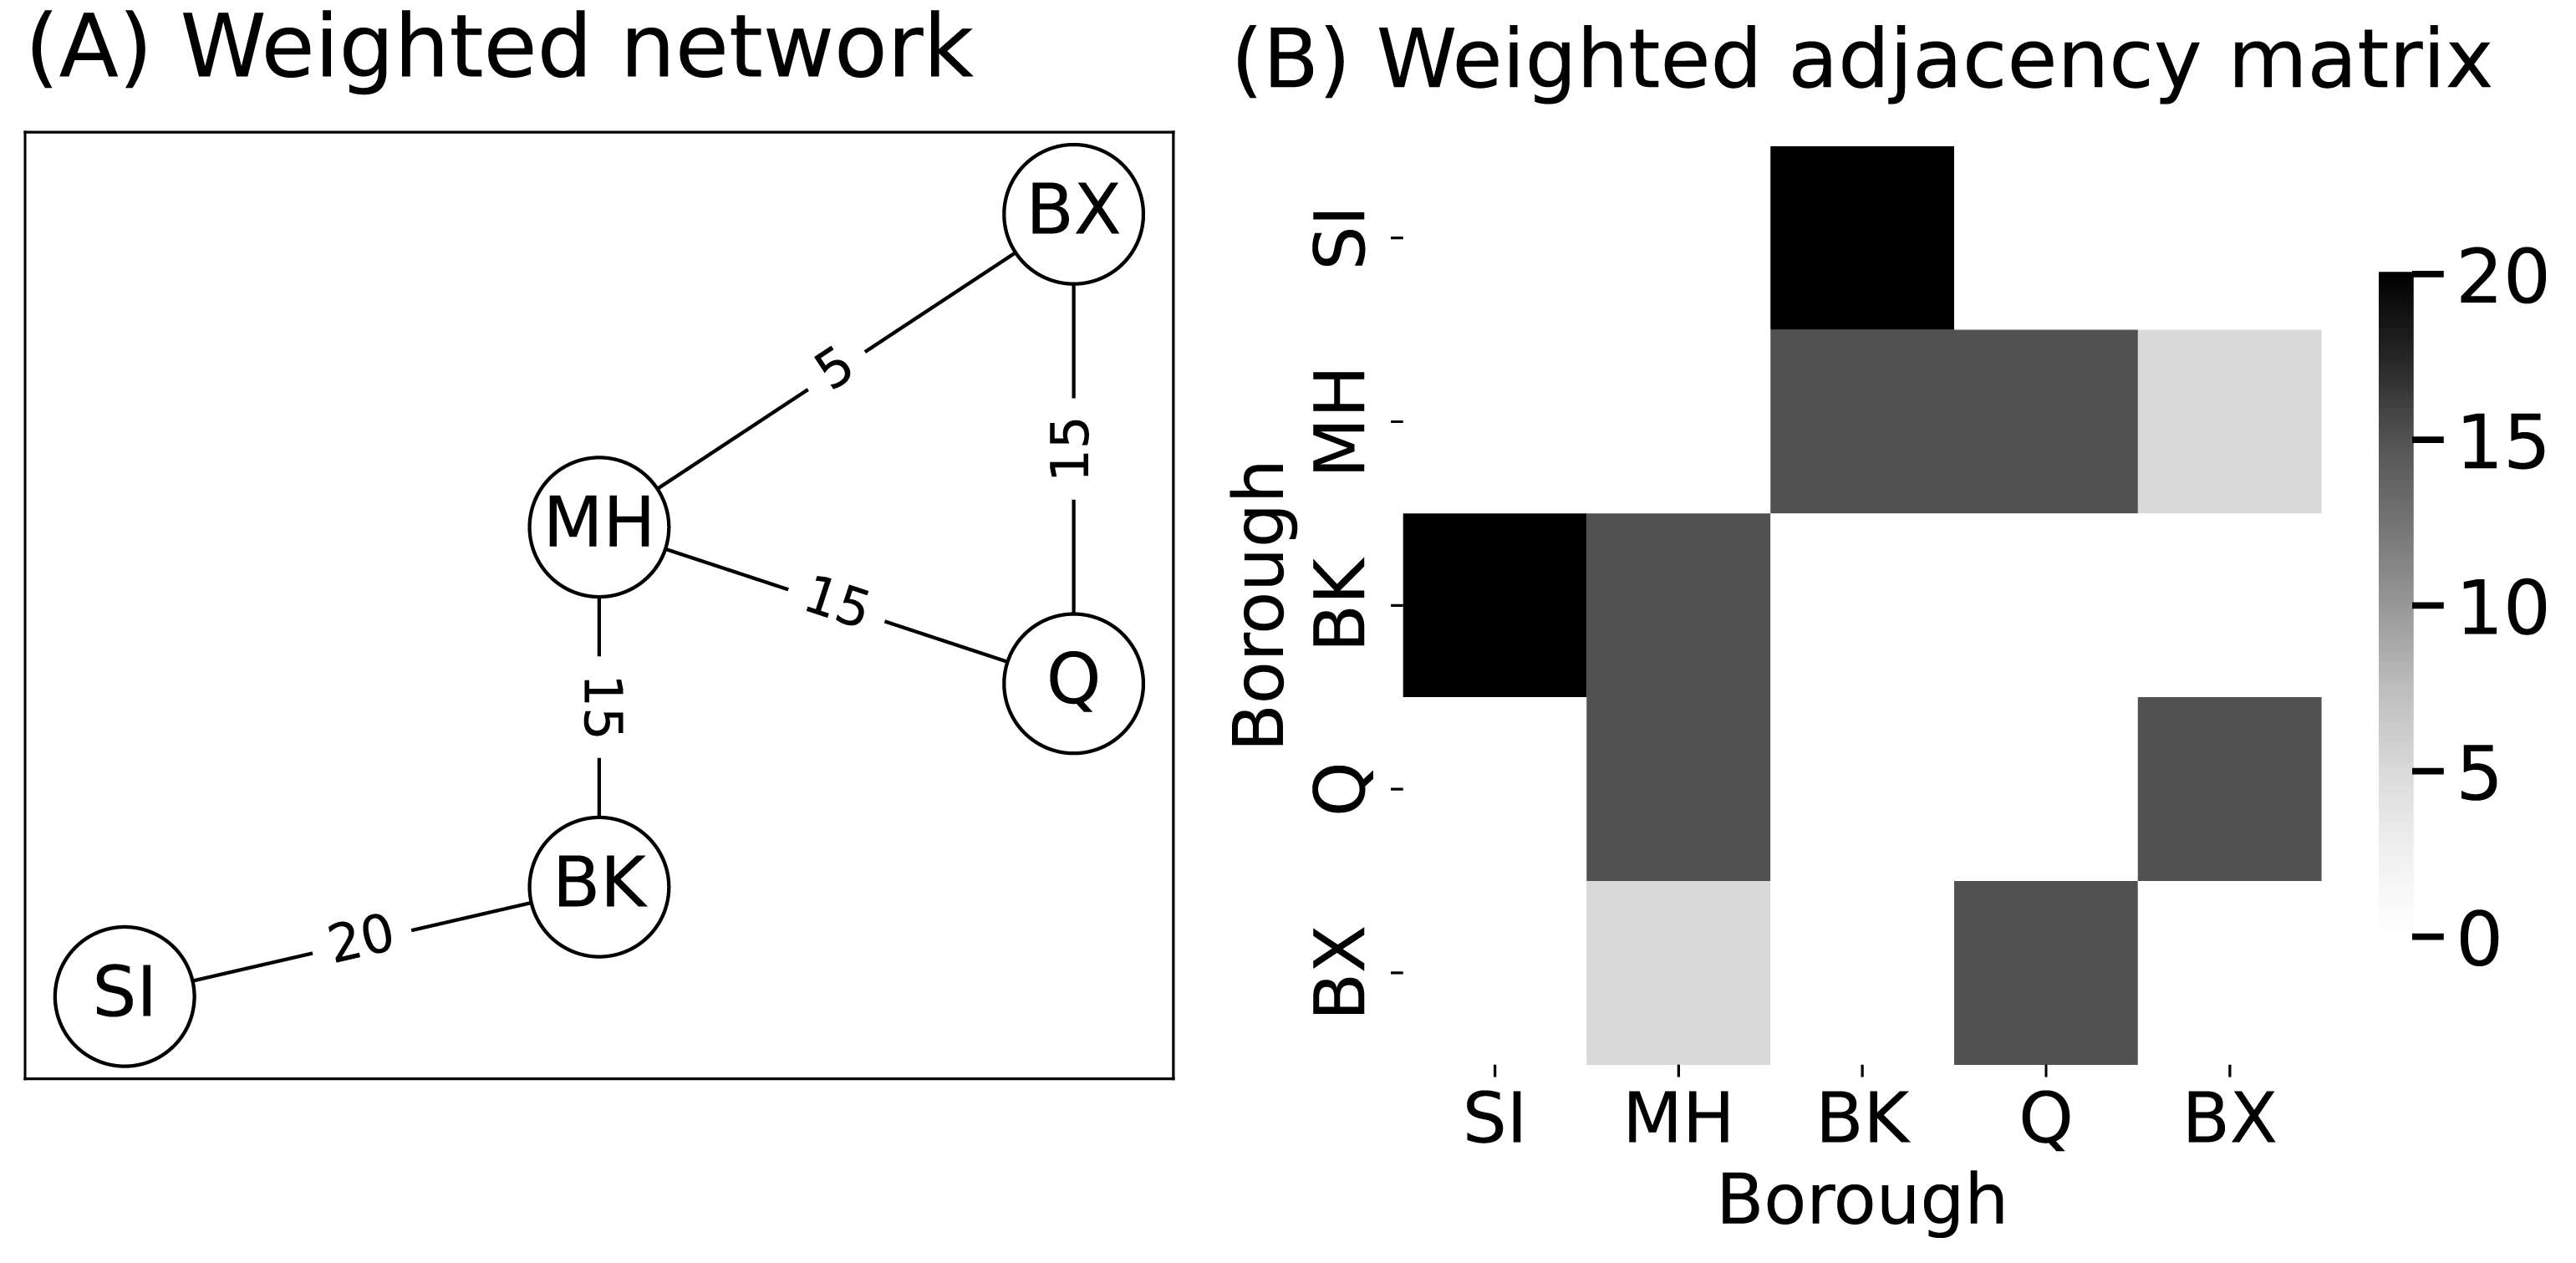
\includegraphics[width=0.8\linewidth]{representations/ch4/Images/weighted.png}
    \caption[Weighted network in New York borough example]{The New York City borough network, where weights indicate the travel times across the indicated bridges. \textbf{(A)} a layout plot for the weighted network, and \textbf{(B)} a heatmap of an adjacency matrix for the weighted network.}
    \label{fig:ch4:weighted}
\end{figure}

\begin{floatingbox}[h]\caption{This book considers {simple networks}}
A \textit{simple network} is loopless, undirected, and unweighted. Most of the examples and techniques you look at in this book are developed in the context of simple networks. Fortunately, this note is largely conceptual, and doesn't really impact much from an implementation perspective. All the techniques and packages you use will make sensible choices, or will directly extend, to cases that fall outside of this particular setup. If your networks don't satisfy one or any of these properties, most of the approaches discussed herein will still work. 

If the technique will not work for the network you have provided, the software package used (such as \texttt{networkx}, \texttt{graspologic}, or \texttt{igraph}) will probably either give you a warning or an explicit error if there is a substantial issue with the network you have provided. That said, when implementing network analysis methods on your own, we strongly encourage you to double check with the documentation to ensure that it is {compatible} with the type of network you are analyzing.
\end{floatingbox}

\subsection{Descriptive Properties of Nodes}

Just like you have many words and properties which describe the network itself, you also have special vocabulary in network machine learning to describe properties about the individual nodes in the network. We'll learn some of the ones here that will come up again later in the book.

\subsubsection{Node neighbors and incidences}

You begin by describing properties of single nodes in a simple network. The simplest property of a network is {adjacency}. A pair of nodes $i$ and $j$ in an undirected network are \textit{neighbors} if an edge exists between them. In terms of the adjacency matrix, two nodes $i$ and $j$ are neighbors if the potential edge $a_{ij}$ is one.

\subsubsection{Node degree quantifies the number of edges}
\label{sec:ch4:prop-net:degree}
The simplest summary statistic for a node is known as the {node degree}. The \textit{node degree} of $i$ in a simple network is the number of nodes with which it is a neighbor. Remember that if two nodes are not neighbors, the adjacency matrix entry corresponding to this {potential} edge takes a value of zero. This means that we can just count the potential edges $a_{ij}$ for a node $i$ to get its degree. We do this by just summing the $i^{th}$ row (or equivalently, if the network is simple, its $i^{th}$ column):

\begin{align}
    d_i &= degree(i) \triangleq \sum_{j = 1}^n a_{ij} = \sum_{j = 1}^n a_{ji}\label{eqn:ch4:degree}
\end{align}

Now you might be thinking, this isn't just counting edges which exist, since it counts {every} potential edge for node $i$. Let's see how that holds up. Remember that if an edge exists, $a_{ij}$ takes a value of $1$, whereas if an edge does not exist, $a_{ij}$ takes a value of $0$. This means that every $a_{ij}$ is either zero or one, so you can write:

\begin{align*}
    d_i &= \sum_{j = 1}^n a_{ij} \\
    &= \sum_{j : a_{ij} = 1} a_{ij} + \sum_{j : a_{ij} = 0}a_{ij} \\
    &= \sum_{j : a_{ij} = 1}1 + 0
\end{align*}
Note that in the left sum, since every $a_{ij}$ is defined to be one, that this is just the number of times that $a_{ij}$ takes a value of one, which is all of the edges that node $i$ touches. The right sum has every $a_{ij}$ defined to be zero, so this is just zero!

For instance, if you consider the node BK in your example, BK touches two edges, indicated in bold in  Figure \ref{fig:ch4:degree}(A), so $degree({BK}) = 2$. When you look at the corresponding adjacency matrix, if you sum the entries for node ${BK}$, you also get two. The entries which would be summed row-wise or column wise for ${BK}$ are shown in black boxes, in Figure \ref{fig:ch4:degree}(B).

\begin{figure}[h]
    \centering
    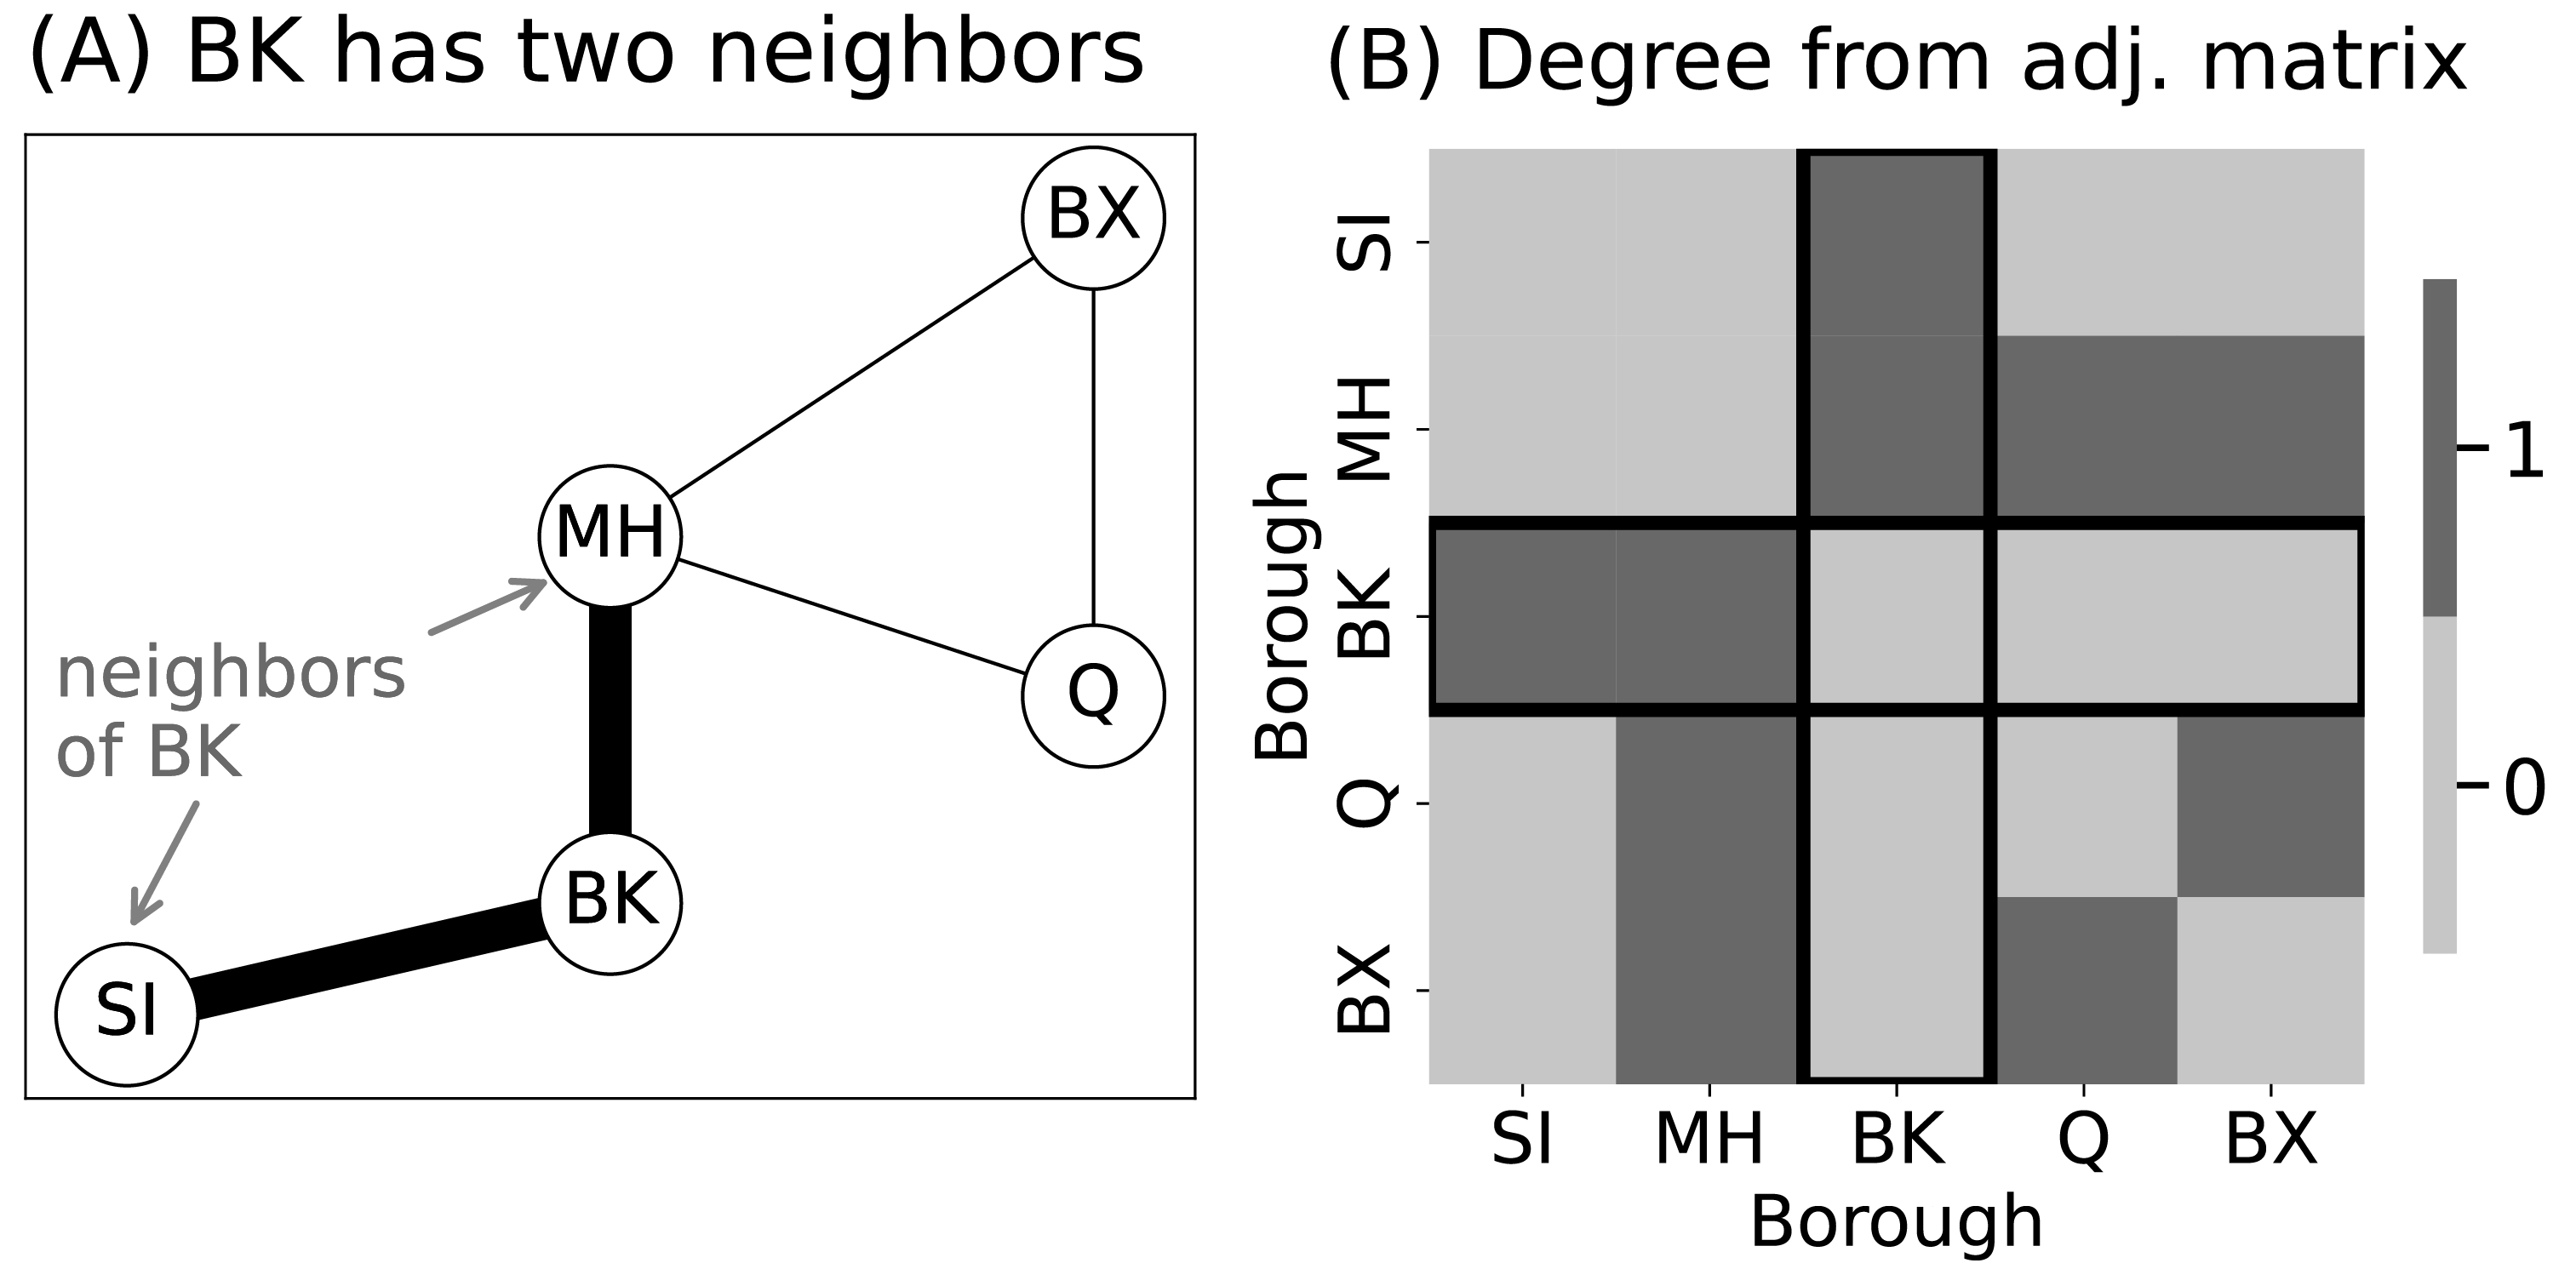
\includegraphics[width=0.8\linewidth]{representations/ch4/Images/degree.png}
    \caption[Deriving node degree from layout and adjacency matrix heatmaps]{A case-study of the BK borough. \textbf{(A)} shows that BK has two neighbors, SI and MH (edges to SI/MH are bold-faced). \textbf{(B)} shows the axes of the adjacency matrix could be summed to derive this fact as well. Note the row/column corresponding to BK (black boxes) has a sum value of two.}
    \label{fig:ch4:degree}
\end{figure}

It really doesn't matter whether you sum row or column-wise, as long as you pick one, if the network is undirected.

\subsubsection{The degree matrix indicates the degrees of each node}

A useful quantity which you will come across in many of the later chapters of this book is called the {degree matrix} of the network. The degree matrix is the {diagonal} matrix:
\begin{align*}
    D &= \begin{bmatrix}
        d_1 & 0 & ... & 0 \\
        0 & \ddots & \ddots& \vdots \\
        \vdots & \ddots & \ddots & 0 \\
        0 & ... & 0 & d_n
    \end{bmatrix}, \;\;\; d_i = degree(i)
\end{align*}
This matrix $D$ is called \textit{diagonal} because all of the entries $d_{ij} = 0$ unless $i = j$. The diagonal entries $d_{ii}$ of the degree matrix are simply the node degrees $degree(i)$ for each node $i$. Using the counting procedure you described above, you can see that the node SI has degree one, the node BK has degree two, the node MH has degree three, the node Q has degree two, and the node BX has degree two. We can compute the degree matrix for an unweighted network by using either of the following commands:

\begin{lstlisting}[style=python]
# summing column-wise
D_column = np.diag(A.sum(axis=0))
# summing row-wise
D_row = np.diag(A.sum(axis=1))
\end{lstlisting}

You can plot the degree matrix using the \texttt{heatmap} utility that we developed for the adjacency matrix.

\paragraph{Degrees for directed networks}

A question you might have in the back of your head is, "what if the network is directed?" When the network is directed, you have two types of degrees, the {in degree} and the {out degree}. The \textit{in degree} of a node $i$ in a directed network is the number of nodes which have edges that go {to} node $i$. Remember that the column of the adjacency matrix, $a_{ji}$, where $j$ indexes all of the nodes of the network, take a value of $1$ if node $j$ has a directed edge from itself to node $i$. This means that to compute the in-degree for node $i$, we just need to sum its column of the adjacency matrix:
\begin{align*}
    d_i^{in} &= \sum_{j = 1}^n a_{ji}
\end{align*}
On the other hand, the \textit{out degree} of a node $i$ is the number of nodes that node $i$ has edges which point to. By the exact same logic, the row of the adjacency matrix $a_{ij}$, where $j$ indexes all of the nodes of the network, takes a value of $1$ if node $i$ has a directed edge from itself to some other node $j$. This means that to compute the out-degree for node $i$, we just need to sum its row of the adjacency matrix:
\begin{align*}
    d_i^{out} &= \sum_{j = 1}^n a_{ij}
\end{align*}
In an undirected network, since $a_{ji} = a_{ij}$ these quantities are equal, which is how we ended up with the nice relationship in the preceding section. 

In a directed network, since there is no concept of a {node degree} like there was for an undirected network, we instead have two degree matrices: the {in-degree matrix} $D^{in}$ and the {out-degree matrix} $D^{out}$. The \textit{in-degree matrix} $D^{in}$ is the matrix whose diagonal entries are the in-degrees of each node $i$ in the network. The \textit{out-degree matrix} $D^{out}$ is the matrix whose diagonal entries are the out-degrees of each node $i$ in the network. 

These can be computed like this:

\begin{lstlisting}[style=python]
# summing column-wise to get out degree
D_out = np.diag(A_dir.sum(axis=0))
# summing row-wise to get in-degree
D_in = np.diag(A_dir.sum(axis=1))
\end{lstlisting}

Incidentally, you can equivalently use matrix multiplication here to get the same results, by matrix-multiplying a vector of ones:

\begin{lstlisting}[style=python]
ones = np.ones(len(A_dir))

D_in_mat = np.diag(A_dir @ ones)
D_out_mat = np.diag(A_dir.T @ ones)

assert np.array_equal(D_in, D_in_mat)
assert np.array_equal(D_out, D_out_mat)
\end{lstlisting}

This is what you'd do in practice, since matrix-multiplication and dot products are highly optimized operations.

\paragraph{Degrees for weighted networks}

If the network is weighted, either weighted and directed or weighted and undirected, all of the logic we've learned so far applies directly. Remember that the adjacency matrix $A$ has entries $a_{ij} = w(i, j)$ if the edge exists between nodes $i$ and $j$ and $0$ otherwise. This means that when we compute the degrees (either the undirected node degree, the in-degree, or the out-degree), we instead sum edge weights when the edge exists, and $0$s otherwise.

\subsection{Network summary statistics tell you useful attributes about networks}

When you learn about networks, it is often valuable to compute properties of the network so that you can get a better understanding of the relationships within it. We will call these properties {network summary statistics}. Although this book will focus more on {learned} representations of networks, summary statistics are a sort of {engineered} representation. Next, we will learn several network summary statistics, and in Section \ref{sec:ch4:net-rep:featurelims}, we will explore the limitations of network summary statistics.


\begin{floatingbox}[h]\caption{Short-hands you will come across in network science}
\label{box:ch4:sums}
When dealing with software packages or technical papers on network data, it is often the case that many authors will favor readability and brevity over writing out things with the most unambiguous notation possible. For this reason, there are a number of short-hands that you are going to want to get familiar with. The most common ones are:
\begin{enumerate}
    \item Double sums $\sum_{i = 1}^n \sum_{j = 1}^n x_{ij}$ will often be abbreviated as $\sum_{i, j = 1}^nx_{ij}$. The reason is that $i$ and $j$ are both summing over the same indexing set $\{1, ..., n\}$, and therefore it is redundant to write it twice.
    \item Likewise, triple sums $\sum_{i = 1}^n \sum_{j = 1}^n \sum_{k = 1}^n x_{ijk}$ will often be abbreviated as $\sum_{i,j,k = 1}^nx_{ijk}$.
    \item You might come across ambiguous sums entirely, such as $\sum_{i,j}x_{ij}$. This would mean to sum over all possible values $i$ and $j$ could take that would make sense when considered with the summand (e.g., the $x_{ij}$ term). For example, if $x_{ij}$ are the entries of an $n \times m$ matrix $X$, this sum would be $\sum_{i = 1}^n \sum_{j = 1}^m x_{ij}$. 
    \item You might come across sums that index inequalities, such as $\sum_{i \neq j}x_{ij}$. This means to consider all possible pairs $(i, j)$ where $i \neq j$. You will come across two of these frequently, for square adjacency matrices $A$:
    \begin{itemize}
        \item $\sum_{i \neq j} a_{ij}$, which means $\sum_{i = 1}^n \sum_{j \neq i}a_{ij}$.
        \item $\sum_{j > i} a_{ij}$, which means $\sum_{i = 1}^n \sum_{j = i + 1}^n a_{ij}$.
    \end{itemize}
\end{enumerate}
\end{floatingbox}


\subsubsection{The network density indicates the fraction of possible edges which exist}
\label{sec:ch4:prop-net:density}
Given the adjacency matrix $A$ of a simple network, what fraction of the possible edges {actually} exist? 

To understand this quantity, first you need to understand how many edges are possible in a network. This is where that ``caveat'' about loopless networks come in in a big way: we need to count in such a way that we don't accidentally assume that self-loops are potential edges; since the self-loops are simply not possible, we need to ignore them. 

You have $n$ total nodes in the network, so $A$ is an $n \times n$ matrix. Therefore, $A$ has $n^2$ total entries. However, it turns out that over {half} of these entries are redundant for simple networks. Since you are assuming the network is simple, the network is by definition loopless. This means that every entry is {by default} $0$ along the diagonal. Since each node $i$ has a corresponding diagonal entry $a_{ii}$, this comes to $n$ entries that you do not need to count. This leaves your total possible number of edges at $n^2$ (the total number of entries in the matrix $A$) minus $n$ (the total number of entries which are automatically $0$), or $n^2 - n = n(n - 1)$. This quantity represents the total number of possible edges which are {not} in the diagonal.

What else are we overcounting? Well, as it turns out, if the network is also {undirected} (which it is, because it is {simple}), every node that is {not} in the diagonal is also being double counted. Why is this? Remember that an undirected network has an adjacency matrix where for every pair of nodes $i$ and $j$, $a_{ij} = a_{ji}$. This means that you overcount the number of possible edges not in the diagonal by a factor of {two}, since each off-diagonal entry $a_{ij}$ has a corresponding entry $a_{ji}$. This leaves the total number of possible edges in the network as $\frac{1}{2}n(n - 1)$, or the total number of possible edges not in the diagonal reduced by a factor of two. This quantity is notated by $\binom n 2$, which is read as ``$n$ {choose} $2$''. You might see this notation arise in the study of {combinatorics}, where it is used to answer the question of, "In how many ways can you {choose} two items from $n$ items?" In the network in Figure \ref{fig:ch4:density}(B), you see all of the {possible} edges indicated. If you count them up, there are $\frac{1}{2}\cdot 5 \cdot (5 - 1) = 10$ possible edges.

Now, how many edges {actually} exist in your network? The sum of all of the entries of $A$ can be represented by the quantity $\sum_{i , j= 1}^n a_{ij}$. For each node $i$, we sum all of the $a_{ij}$, and then we add these across all of the nodes. Remember that $A$ is loopless, so you don't need to count the diagonal entries. This brings your quantity to $\sum_{i \neq j}a_{ij}$, since you don't need to count any edges along the diagonal of $A$. Next, remember that if an edge in $A$ exists between nodes $i$ and $j$, that {both} $a_{ij}$ and $a_{ji}$ take the value of $1$, due to the undirected property. To obtain the edge count of $A$, that you only need to count {either} $a_{ij}$ {or} $a_{ji}$. Somewhat arbitrarily in this book, we will always count the entries $a_{ij}$ in the upper triangle of $A$, which are the entries where $j > i$. This brings your quantity to $\sum_{j > i} a_{ij}$. 

The edges in your network will be indicated in Figure \ref{fig:ch4:density}(A), of which there are $5$ total. 

\begin{figure}[h]
    \centering
    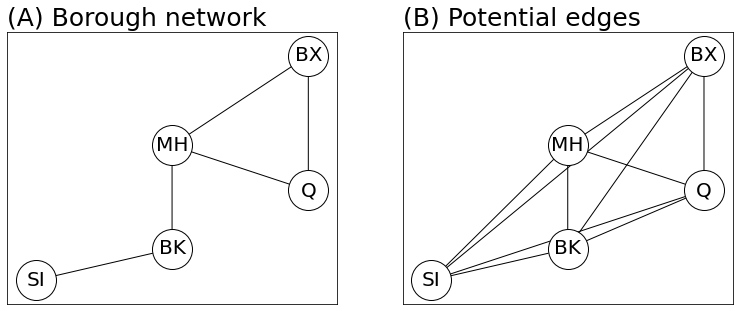
\includegraphics[width=0.8\linewidth]{representations/ch4/Images/density.png}
    \caption[Visualizing network density]{\textbf{(A)} The New York Borough network. The actual edges are shown. \textbf{(B)} The New York Borough network with all possible potential edges.}
    \label{fig:ch4:density}
\end{figure}

To put it all together, the \textit{network density} indicates the {density of edges} which are present in the network. For a simple network, the network density can be defined as the ratio between the total number of edges in $A$ and the total number of edges possible in $A$:
\begin{align}
    density(A) &= \frac{\sum_{j > i}a_{ij}}{\binom n 2} = \frac{2\sum_{j > i}a_{ij}}{n(n - 1)}
    \label{eqn:ch4:netdens}
\end{align}
In your example, this is simply the ratio of edges which {actually} exist to edges which could {possibly} exist, which is $\frac{5}{10} = 0.5$. You can compute the network density via \texttt{networkx} using the function \texttt{density()}:

\begin{lstlisting}[style=python]
nx.density(G)
# 0.5
\end{lstlisting}
In a simple network, there are a few additional ways you might see this equation written. Notice that the following inequality is true, by definition of a simple network:
\begin{align*}
    \sum_{i,j = 1}^n a_{ij} &= \sum_{j > i}a_{ij} + \sum_{i > j}a_{ij} + \sum_{i = 1}^n a_{ii} \\
    &= \sum_{j > i}a_{ij}+ \sum_{i > j}a_{ij} + 0,
\end{align*}
which is because the network is loopless (so the diagonal is $0$). Further, remember that $a_{ij} = a_{ji}$, which means that the first term is {exactly} equal to the second term, so:
\begin{align*}
    \sum_{i,j = 1}^n a_{ij} &= \sum_{j > i}a_{ij}+ \sum_{i > j}a_{ij} \\
    &= \sum_{j > i}a_{ij}+ \sum_{j > i}a_{ij} = 2\sum_{j > i}a_{ij} \\
    \Rightarrow \sum_{j > i}a_{ij} &= \frac{1}{2}\sum_{i,j = 1}^n a_{ij}
\end{align*}
This gives us the useful relationship that we can re-write the density even more simply, by plugging this relationship into Equation \eqref{eqn:ch4:netdens} as:
\begin{align*}
    density(A) &= \frac{\frac{1}{2}\sum_{i = 1}^n \sum_{j = 1}^n a_{ij}}{\binom n 2} = \frac{\sum_{i = 1}^n \sum_{j = 1}^n a_{ij}}{n(n - 1)}
\end{align*}
We wrote out the double sum here because there is a key relationship that we want to point out. Notice that the inner-most sum is just computing the degree $d_i$ of each node $i$, because $d_i = \sum_{j = 1}^n a_{ij}$ in an undirected network. This means that:
\begin{align}
    density(A) &= \frac{\frac{1}{2}\sum_{i = 1}^n d_i}{\binom n 2} = \frac{\sum_{i = 1}^n d_i}{n(n - 1)} \label{eqn:ch4:density_degree}
\end{align}
As a final note, notice that $\frac{1}{n}\sum_{i = 1}^n d_i$ is the \textit{average degree} over sll of the $n$ nodes in the network. We will typically abbreviate this quantity using the symbol $d$. Using this fact with the right-most equality in Equation \eqref{eqn:ch4:density_degree}, we see that:
\begin{align*}
    density(A) &= \frac{d}{n - 1}.
\end{align*}
In this sense, the density can be conceptualized as the average degree of each node in the network, divided by the maximum possible degree each node could have (which, in a simple network, is $n-1$, since a node could at most have an edge to the other $n-1$ nodes in the network). This concept will become handy when we think about sparsity in Section \ref{sec:ch10:sparsity}.


\subsubsection{The clustering coefficient indicates how much nodes tend to cluster together}
\label{sec:ch4:prop-net:clustering}

The clustering coefficient indicates the fraction of triplets of nodes which are closed. What the heck is that? Let's look at only Brooklyn, Manhattan, Queens, and the Bronx, and temporarily ignore Staten Island:

\begin{lstlisting}[style=python]
G_clus = nx.Graph()

G_clus.add_node("MH", pos=(4,4))
G_clus.add_node("BK", pos=(4,1.7))
G_clus.add_node("Q", pos=(6,3))
G_clus.add_node("BX", pos=(6,6))


pos = nx.get_node_attributes(G, 'pos')
G_clus.add_edge("MH", "BX")
G_clus.add_edge("MH", "BK")
G_clus.add_edge("MH", "Q")
G_clus.add_edge("Q", "BX")

nx.draw_networkx(G_clus, with_labels=True, node_color="black", pos=pos,
                 font_color="white", edge_color="black")
\end{lstlisting}
The plotted result is shown in \ref{fig:ch4:subnet}(B).

To begin to define the clustering coefficient, you first must understand what a {triplet} is. A \textit{triplet} is an ordered tuple of three nodes which are connected by two or three edges. Note that a tuple of three nodes to be a triplet, you must be able to travel from one end of the triplet to the other along a contiguous path. The triplets are {closed} if there are three edges, and {open} if there are only two edges. For instance, in the above network, you have the following triplets of nodes:
\begin{enumerate}
    \item Open triplets between Bronx, Manhattan, and Brooklyn: (BX, MH, BK), (BK, MH, BX),
    \item Open triplets between Manhattan, Queens, and Brooklyn: (BK, MH, Q), (Q, MH, BK),
    \item Closed triplets between Bronx, Manhattan, and Queens: (BX, MH, Q), (BX, Q, MH), (MH, BX, Q), (MH, Q, BX), (Q, BX, MH), (Q, MH, BX),
\end{enumerate}

To clarify a fine technical point of open triplets, we do not count (BK, Q, MH) as a triplet because there is no edge from BK to Q. You must be able to go from the first node to the second to the third along edges that exist in the network in order for a triple of nodes to count as a triplet. No triplets are possible between Brooklyn, Bronx, and Queens, because only a single edge exists between the three of them. In your example, there are six closed triplets amongst the nodes (delineated in number 3. above), and there are 4 open triplets (delineated in numbers 1. and 2. above). The global clustering coefficient (or transitivity) is defined as:

\begin{align*}
    C &= \frac{\text{number of closed triplets}}{\text{number of closed triplets} + \text{number of open triplets}}
\end{align*}
In our example, this comes to $C = \frac{6}{6 + 4} = 0.6$. This equation can also be understood in terms of the adjacency matrix. Note that if a triplet between nodes $i$, $j$, and $k$ is closed, then all three of the potential edges $a_{ij}$, $a_{jk}$, and $a_{ki}$ have a value of $1$. Therefore, if you could the number of times that $a_{ij}a_{jk}a_{ki} = 1$, you also count the number of closed triplets! This means that the number of closed triplets can be expressed as $\sum_{i,j,k = 1}^na_{ij}a_{jk}a_{ki}$. 

Further, note that for a given node $i$, you can find an arbitrary triplet (either open or closed) through the following procedure.
1. Pick a single neighbor $j$ for node $i$. Note that the node $i$ has a number of neighbors equal to $degree(i) = d_i$, so there are $d_i$ possible neighbors to choose from.
2. Pick a different neighbor $k$ for node $i$. Note that since node $i$ had $d_i$ neighbors, it has $d_i - 1$ neighbors that are not node $j$.
3. Since you know that nodes $j$ and $k$ are both neighbors of node $i$, you know that $a_{ij}$ and $a_{ik}$ both have values of one, and therefore the edges $(i, j)$ and $(i, k)$ exist. Therefore, the tuple of nodes $(i, j, k)$ is a triplet, because {at least} two edges exist amongst the three nodes. This tuple is closed if the edge $(j, k)$ exists, and open if the edge $(j, k)$ does not exist.
4. Therefore, there are $d_i (d_i - 1)$ triplets in which node $i$ is the leading node of the triplet.

As it turns out, since triplets are {ordered tuples}, you can repeat this procedure for all nodes, and if you count how many triplets you get in total, you get the {total number of triplets} for the entire network. Therefore, the number of open and closed triplets in the network is the quantity $\sum_i d_i (d_i - 1)$.  Then you could express the clustering coefficient in terms of the adjacency matrix as:

\begin{align*}
    C &= \frac{\sum_{i,j,k = 1}^n a_{ij}a_{jk}a_{ki}}{\sum_{i = 1}^n d_i (d_i - 1)}
\end{align*}
Which gives you an expression to implement programmatically. You can compute the clustering coefficient via \texttt{networkx} using:

\begin{lstlisting}[style=python]
nx.transitivity(G_clus)
# 0.6
\end{lstlisting}


\subsubsection{The path length describes how far two nodes are}
\label{sec:ch4:prop-net:path}
How many bridges would you need to cross to get from Staten Island to Bronx? This concept relates directly to the concept of the {path length} in a network. A \textit{path} between two nodes $i$ and $j$ is a sequence of edges which starts at node $i$, and traverses through other nodes in the network until reaching node $j$. Two nodes are described as \textit{connected} if a path exists between them. The \textit{path length} is the number of edges in the path. For instance, if you remember your network from the New York example, you could get from Staten Island to Bronx in two possible ways, indicated in in (B) and (C) in Figure \ref{fig:ch4:path}.

\begin{figure}[h]
    \centering
    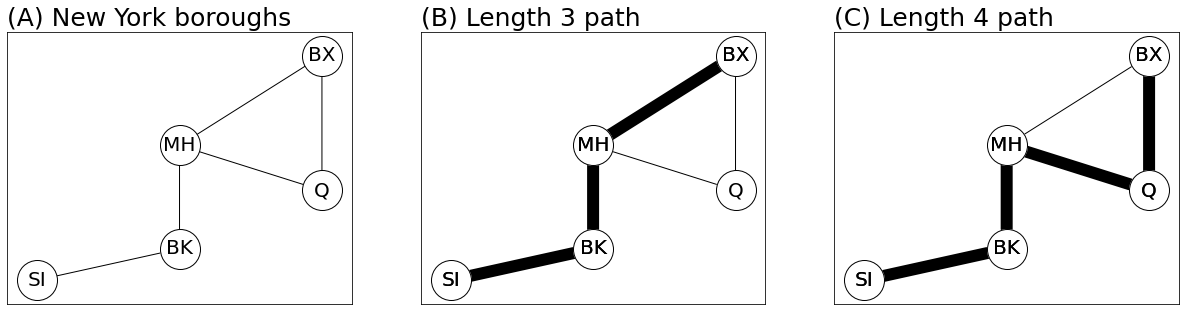
\includegraphics[width=\linewidth]{representations/ch4/Images/path.png}
    \caption[Path length in New York boroughs]{\textbf{(A)} The New York boroughs. \textbf{(B)} A length $3$ path from SI to BX. \textbf{(C)} A length $4$ path from SI to BX.}
    \label{fig:ch4:path}
\end{figure}
In this case, there are only two paths from SI to BX which do not visit the same node more than once, but in a larger network, there may be {many} possible paths from one node to another. For this reason, you will usually be interested in one particular path, the {shortest path}. The \textit{shortest path length} or \textit{distance} between nodes $i$ and $j$ is the path with the smallest path length that connects nodes $i$ and $j$. In your example, the shortest path is indicated by Figure \ref{fig:ch4:path}(B), and the shortest path length is therefore three.  If it is not possible to get from node $i$ to node $j$ using edges of the network, the shortest path length is defined to be infinite. The shortest path between nodes $i$ and $j$ will often be abbreviated using the notation $l_{ij}$.

A common statistic often calculated is the {distance matrix} for the network $L$, which is the $n \times n$ matrix whose entries $l_{ij}$ are the shortest path lengths between all pairs of nodes in the network. For your New York example, you can compute and visualize the distance matrix using:

\begin{lstlisting}[style=python]
L = nx.floyd_warshall_numpy(G)
heatmap(L, title="Distance matrix",  xticklabels=["SI", "MH", "BK", "Q", "BX"],
        yticklabels=["SI", "MH", "BK", "Q", "BX"], xtitle="Borough", ytitle="Borough")
\end{lstlisting}
Another common statistic you can compute using the distance matrix is the {average shortest path length}. The average shortest path length $l$ of a simple network is simply the average of all of the shortest paths between two distinct nodes $i$ and $j$ of the distance matrix:
\begin{align*}
    l &= \frac{1}{n(n - 1)}\sum_{i \neq j} l_{ij}
\end{align*}
The normalizing factor here is $n(n - 1)$ because the sum $\sum_{i \neq j}$ is short-hand for the double-sum $\sum_{i = 1}^n \sum_{j \neq i}$. Notice that the left-most sum has $n$ terms, and for each node $i$, there are $n-1$ other possible values that $j$ can take where $j \neq i$. This means that we are summing $n-1$ terms $n$ times (which is $n (n - 1)$). 

\paragraph{Paths in directed networks}

If the network is directed, the interpretation of a path is exactly the same, except you have to be careful to account for the directionality when finding paths from one node to the next. For instance, in Figure \ref{fig:ch4:directed}(B), there {is} a path from the nodes MH, Q, BX to SI or BK, but there are {no} paths from SI or BK to MH, Q, BX (as the bridge from BK to MH is out of service in the example).

\subsection{Subnetworks are subsets of larger networks}
\label{sec:ch4:prop-net:subnetwork}
When you think of an entire network, it is often useful to consider it in smaller bits. For instance, when you were looking at the clustering coefficient, you found it useful to break out the nodes {BK, Q, BX, MH} so you could count triplets, like we did in Section \ref{sec:ch4:prop-net:clustering}. 

This portion of the network is called a {subnetwork}. A \textit{subnetwork} is a network whose nodes and edges are {subsets} of the nodes and edges for another network. In this case, the  network toplogy of the New York example is $(\mathcal V, \mathcal E)$ defined by the sets:

\begin{enumerate}
    \item The nodes $V$: $\{SI, BK, Q, MH, BX\}$, and
    \item The edges $E$: $\left\{(SI, BK), (BK, MH), (MH, Q), (MH, BX), (Q, BX)\right\}$.
\end{enumerate}

and the subnetwork (which removed Staten Island, SI) we looked at above is the network:

\begin{enumerate}
    \item The nodes $V_s$: $\{BK, Q, MH, BX\}$, and
    \item The edges $E_s$: $\left\{(BK, MH), (MH, Q), (MH, BX), (Q, BX)\right\}$.
\end{enumerate}

As you can see, the subnetwork with nodes and edges $(V_s, E_s)$ is such that every element in $V_s$ is an element of $V$, and therefore the nodes of the subnetwork are a subset of the nodes of the complete network. Further, every element in $E_s$ is an element of $E$, and therefore the edges of the subnetwork are a subset of the edges of the complete network. So the subnetwork $(V_s, E_s)$ is a subnetwork of the network $(V, E)$. This particular subnetwork can be described further as an \textit{induced} subnetwork. A subnetwork of a network is \textit{induced} by a set of nodes if the following conditions hold:

\begin{enumerate}
    \item The nodes $V_s$ are a subset of the nodes of the network $V$, and
    \item The edges $E_s$ consist of {all} of the edges from the original network where both of the corresponding nodes are in $V_s$.
\end{enumerate} 

An example of the induced subnetwork we showed above is shown in Figure \ref{fig:ch4:subnet}(B). To see an example of a subnetwork which is {not} an induced subnetwork, check out Figure \ref{fig:ch4:subnet}(C). Try to determine why this subnetwork is not induced. You can create an induced subnetwork (in this case, by BK, MH, Q, BX) using networkx:

\begin{lstlisting}[style=python]
G_sg = G.subgraph(["BK", "MH", "Q", "BX"]).copy()
nx.draw_networkx(G_sg, with_labels=True, node_color="black", pos=pos,
                 font_color="white", edge_color="black")
\end{lstlisting}

\begin{figure}[h]
    \centering
    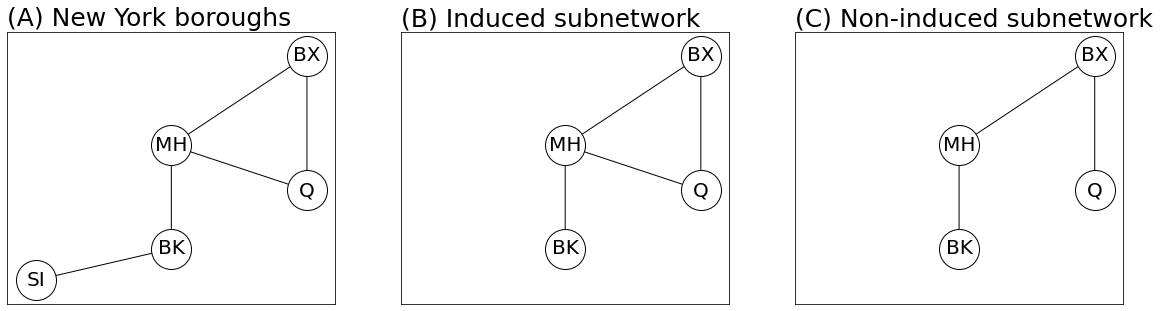
\includegraphics[width=\linewidth]{representations/ch4/Images/subnet.png}
    \caption[New York boroughs example]{\textbf{(A)} The New York Borough example. \textbf{(B)} The subnetwork induced by the node set \{BX, MH, Q, BX\}. This is also the example that we used to study clustering. \textbf{(C)} A subnetwork that is not an induced subnetwork.}
    \label{fig:ch4:subnet}
\end{figure}

\paragraph*{Representing subnetworks}
Notice that a subnetwork is a collection of nodes and edges defined on these nodes. Therefore, a subnetwork is itself also a network. This means that we could still represent a subnetwork using an adjacency matrix, with the caveat that the number of rows and columns might not be the same (since the nodes of a subnetwork are a subset of the nodes of the network) and the density might change (since the edges of a subnetwork are a subset of the edges of the network).

Let's think about why this matters.

\paragraph*{A caveat with the adjacency matrix of subnetworks}
Let's imagine that you have a simple network with the adjacency matrix $A$:
\begin{align*}
    A = \begin{bmatrix}
        0 & 0 & 0 \\
        0 & 0 & 1 \\
        0 & 1 & 0
    \end{bmatrix}
\end{align*}
And you consider a subnetwork that is induced by nodes \{2, 3\}. The induced subnetwork would have an adjacency matrix that looks like this:
\begin{align*}
    A_s = \begin{bmatrix}
        0 & 1 \\
        1 & 0
    \end{bmatrix}
\end{align*}
The key idea here is that, if you ignore the structure of the network when we do this, and conceptualize an induced subnetwork as a {deletion} of rows and columns, it becomes very difficult to figure out (later on in your analysis) which node is which. For instance, in your initial network, you might have also had a vector with $3$ elements (one for each node) that contained useful information about the nodes that you want to use later in your analysis. If you discard which nodes were included in your subnetwork, it will be very difficult (later in the analysis) to decipher which node is associated with which piece of information in your vector. For this reason, whenever you compute a subnetwork, we would {strongly} recommend that you make a note of it somewhere and store the nodes from the initial network that were retained in the subnetwork, so that you don't end up confused later on.

A particular induced subnetwork that you will often be concerned with is known as the largest connected component (LCC). 


\subsubsection{The largest connected component (LCC) is the largest subnetwork of connected nodes}
\label{sec:ch4:prop-net:lcc}
To define the largest connected component, we'll need to modify our example slightly. Let's say your network also includes the Boston area, and you have two new nodes, Boston (BO) and Cambridge (CA). Boston and Cambridge have several bridges between one another, so an edge exists between them. However, there are no bridges between boroughs of New York and the Boston area, so there are no edges from nodes in the Boston area to nodes in the New York area. Let's see how we would add this programmatically:

\begin{lstlisting}[style=python]
G_withbos = deepcopy(G)
G_withbos.add_node("BO", pos=(8, 6))
G_withbos.add_node("CA", pos=(8, 8))
G_withbos.add_edge("BO", "CA")
# fetch positions with boston and cambridge added
pos = nx.get_node_attributes(G_with_bos, 'pos')
# plot
nx.draw_networkx(G_withbos, with_labels=True, node_color="black", pos=pos,
                font_color="white", edge_color="black")
\end{lstlisting}

We visualize the network with Boston and Cambridge in Figure \ref{fig:ch4:lcc}(A). 

The entire network can be described by the sets:
\begin{enumerate}
    \item $\mathcal V = \{SI, MH, BK, BX, Q, CA, BO\}$, and
    \item $\mathcal E = \{(SI, BK), (MH, BK), (MH, Q), (MH, BX), (MX, Q), (CA, BO)\}$.
\end{enumerate}

Notice that you have two distinct sets of nodes, those of New York and those of Boston, which are {only} connected amongst one another. Formally, these two sets of nodes can be described as inducing {connected components} of the network topology $(\mathcal V, \mathcal E)$. A \textit{connected component} is an induced subnetwork in which any two nodes are connected to each other by a path through the network. The two connected components are the New York induced subnetwork:

\begin{enumerate}
    \item The nodes $\mathcal V_N$: $\{SI, BK, Q, MH, BX\}$, and
    \item The edges $\mathcal E_N$: $\left\{(SI, BK), (BK, MH), (MH, Q), (MH, BX), (Q, BX)\right\}$.
\end{enumerate}

and the Boston induced subnetwork:
\begin{enumerate}
    \item The nodes $\mathcal V_B$: $\{CA, BO\}$, and
    \item The edges $\mathcal E_B$: $\left\{(CA, BO)\right\}$.
\end{enumerate}

We plot each individually in Figure \ref{fig:ch4:lcc}(B) and Figure \ref{fig:ch4:lcc}(C). If the network and the largest connected component are equivalent, we can omit the term {component}, and just say that the network is \textit{connected}.

\begin{figure}[h]
    \centering
    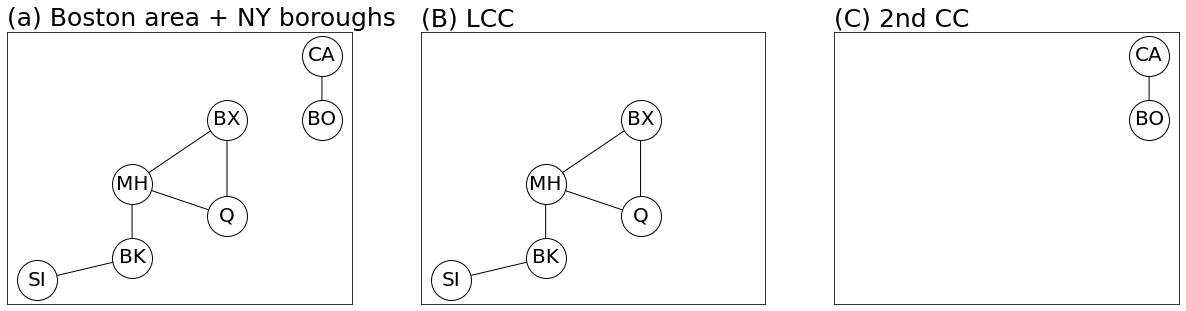
\includegraphics[width=\linewidth]{representations/ch4/Images/lcc.png}
    \caption[Connected Components]{\textbf{(A)} shows the New York boroughs with the added nodes for Boston and Cambridge. \textbf{(B)} shows the connected component induced by the boroughs of New York, which is also the LCC. \textbf{(C)} shows the connected component induced by Boston and Cambridge.}
    \label{fig:ch4:lcc}
\end{figure}
The \textit{largest connected component} (LCC) of a network is the connected component with the most nodes. In your example, the New York connected component has five nodes, whereas the Boston connected component has two nodes. Therefore, the New York connected component is the LCC of this simple network. You can compute the connected components and plot the largest connected component using \texttt{networkx} like this:

\begin{lstlisting}[style=python]
# returns a list of connected components, ordered 
# by decreasing size (#nodes)
cc_withbos = nx.connected_components(G_withbos)
# return the connected components, as networks
CC_nets = [G_withbos.subgraph(cc).copy() for cc in cc_withbos]

# plot the LCC
nx.draw_networkx(CC_nets[0], with_labels=True, node_color="black", pos=pos,
                font_color="white", edge_color="black")
\end{lstlisting}

A lot of times, when you are dealing with networks, they might already be in adjacency matrices. You can pass adjacency matrices directly into \texttt{graspologic} to obtain a LCC using:
\begin{lstlisting}
from graspologic.utils import largest_connected_component as lcc

A_withbos = nx.to_numpy_array(G_withbos)
A_lcc, retained_nodes = lcc(A_withbos, return_inds=True)
\end{lstlisting}
This is one of the {easiest} times for the caveat that we mentioned about subnetworks to arise. The \texttt{return\_inds} argument returns the rows/columns of \texttt{A\_withbos} that were retained for the LCC. The default functionality is to {not} return these indices, so proceed with caution!

\subsubsection{Connected components in directed networks}

The \textit{largest connected component} (LCC) of a network is the connected component with the most nodes. In your example, the New York connected component has five nodes, whereas the Boston connected component has two nodes. Therefore, the New York connected component is the LCC of this simple network.

Like the degree compared to the in- and out- degrees, for directed networks, connected components for directed networks need to be defined a little bit differently. A directed subnetwork is \textit{strongly connected} if directed paths exist between every pair of nodes in the subnetwork. 

A directed subnetwork is \textit{weakly connected} if the underlying directionalities are ignored, and the resulting undirected subnetwork is a connected component. Figure \ref{fig:ch4:directed}(C) shows an example of a strongly connected network, because you can travel along a path from each node to every other node in the network. On the other hand, Figure \ref{fig:ch4:directed}(B) shows an example of a weakly connected component when the bridge from MH to BK is out of service. This is because there is no longer a way to follow a path from SI or BK to MH, Q, and BX. When we ignore the arrows entirely, the resulting undirected network is still connected, as shown in Figure \ref{fig:ch4:directed}(A).


\newpage